\let\negmedspace\undefined
\let\negthickspace\undefined
\documentclass[journal]{IEEEtran}
\usepackage[a5paper, margin=10mm, onecolumn]{geometry}
\usepackage{lmodern} % Ensure lmodern is loaded for pdflatex
\usepackage{tfrupee} % Include tfrupee package

\setlength{\headheight}{1cm} % Set the height of the header box
\setlength{\headsep}{0mm}     % Set the distance between the header box and the top of the text

\usepackage{gvv-book}
\usepackage{gvv}
\usepackage{cite}
\usepackage{amsmath,amssymb,amsfonts,amsthm}
\usepackage{algorithmic}
\usepackage{graphicx}
\usepackage{textcomp}
\usepackage{xcolor}
\usepackage{txfonts}
\usepackage{listings}
\usepackage{enumitem}
\usepackage{mathtools}
\usepackage{gensymb}
\usepackage{comment}
\usepackage[breaklinks=true]{hyperref}
\usepackage{tkz-euclide} 
\usepackage{listings}
\usepackage{gvv}                                        
\def\inputGnumericTable{}                                 
\usepackage[latin1]{inputenc}                                
\usepackage{color}                                            
\usepackage{array}                                            
\usepackage{longtable}                                       
\usepackage{calc}                                             
\usepackage{multirow}                                         
\usepackage{hhline}                                           
\usepackage{ifthen}                                           
\usepackage{lscape}
\begin{document}

\bibliographystyle{IEEEtran}
\vspace{3cm}

\title{NCERT-8.2.7}
\author{EE24BTECH11036 - Krishna Patil}
% \maketitle
% \newpage
% \bigskip
{\let\newpage\relax\maketitle}
\textbf{Question : } Calculate the area bounded by the curves $y^2 = 4x$ and $y = 2x$ . \\ \\
\solution \\
\textbf{(a) Theoretical Solution : }
\begin{enumerate}
    \item \textbf{Find Points of Intersection:} \\  
    To find the points of intersection, solve the system of equations:  
    \begin{align}
        y^2 &= 4x, \\
        y &= 2x.
    \end{align}

    Substitute $y = 2x$ into $y^2 = 4x$:  
    \begin{align}
        \brak{2x}^2 &= 4x, \\
        4x^2 &= 4x, \\
        x \brak{x - 1} &= 0.
    \end{align}

    Thus, $x = 0$ or $x = 1$.  
    For $x = 0$ $y = 2 \cdot 0 = 0$, so one point is $\brak{0, 0}$.  
    For $x = 1$, $y = 2 \cdot 1 = 2$, so the other point is $\brak{1, 2}$.  
    Therefore, the curves intersect at $\brak{0, 0}$ and $\brak{1, 2}$. \\

    \item \textbf{Set Up the Integral:}  \\
    The parabola is $y^2 = 4x \implies x = \frac{y^2}{4}$, and the line is $x = \frac{y}{2}$.  
    To calculate the area, we integrate the difference between the parabola and the line in terms of $y$, from $y = 0$ to $y = 2$:
    \begin{align}
        \text{Area} = \int_{y=0}^{y=2} \brak{ \frac{y}{2} - \frac{y^2}{4} } \, dy.
    \end{align} \\

    \item \textbf{Evaluate the Integral:}  \\
    Expand the integral:
    \begin{align}
        \text{Area} = \int_{0}^{2} \frac{y}{2} \, dy - \int_{0}^{2} \frac{y^2}{4} \, dy.
    \end{align}

    First term:
    \begin{align}
        \int_{0}^{2} \frac{y}{2} \, dy &= \frac{1}{2} \int_{0}^{2} y \, dy = \frac{1}{2} \brak{ \frac{y^2}{2} }_{0}^{2} = \frac{1}{2} \cdot \frac{4}{2} = 1.
    \end{align}

    Second term:
    \begin{align}
        \int_{0}^{2} \frac{y^2}{4} \, dy &= \frac{1}{4} \int_{0}^{2} y^2 \, dy = \frac{1}{4} \brak{ \frac{y^3}{3} }_{0}^{2} = \frac{1}{4} \cdot \frac{8}{3} = \frac{2}{3}.
    \end{align}

    Now subtract:
    \begin{align}
        \text{Area} = 1 - \frac{2}{3} = \frac{3}{3} - \frac{2}{3} = \frac{1}{3}.
    \end{align} \\
    
\textbf{(b) Numerical Solution / Simulation : } \\
\item The integral representing the area is:
    \begin{align}
    A = \int_{y=0}^{y=2} \brak{-x_{\text{parabola}} + x_{\text{line}}} \, dy.
    \end{align}
    From the equations of the curves:
    \begin{align}
    x_{\text{parabola}} &= \frac{y^2}{4}, \\
    x_{\text{line}} &= \frac{y}{2}.
    \end{align}
    Substituting:
    \begin{align}
    A = \int_{0}^{2} \brak{-\frac{y^2}{4} + \frac{y}{2}} \, dy.
    \end{align} \\

    \item Divide the interval $[0, 2]$ into $n$ equal subintervals. Each subinterval has a width:
    \begin{align}
    h = \frac{2}{n}.
    \end{align}
    Let the points be:
    \begin{align}
    y_0 = 0, \, y_1 = h, \, y_2 = 2h, \, \dots, \, y_n = 2.
    \end{align}
    At each point $y_i$, the function to evaluate is:
    \begin{align}
    f(y_i) = -\frac{y_i^2}{4} + \frac{y_i}{2}.
    \end{align} \\

    \item Using the trapezoidal rule, the approximation for the area is:
    \begin{align}
    A \approx \frac{h}{2} \brak{f(y_0) + 2f(y_1) + 2f(y_2) + \dots + 2f(y_{n-1}) + f(y_n)}.
    \end{align} \\

    \item Substitute the expression for $f(y_i)$:
    \begin{align}
    f(y_i) = -\frac{(i \cdot h)^2}{4} + \frac{i \cdot h}{2}.
    \end{align}
    Hence:
    \begin{align}
    A &\approx \frac{h}{2} \brak{\brak{-\frac{y_0^2}{4} + \frac{y_0}{2}} 
    + 2 \sum_{i=1}^{n-1} \brak{-\frac{(i \cdot h)^2}{4} + \frac{i \cdot h}{2}} 
    + \brak{-\frac{y_n^2}{4} + \frac{y_n}{2}}}.
    \end{align} \\

    \item Simplify the terms:
    - At $y_0 = 0$: $f(y_0) = 0$. \\
    - At $y_n = 2$: 
    \begin{align}
    f(y_n) = -\frac{2^2}{4} + \frac{2}{2} = 1 - 1 = 0.
    \end{align}
    Thus:
    \begin{align}
    A \approx \frac{h}{2} \cdot 2 \sum_{i=1}^{n-1} \brak{-\frac{(i \cdot h)^2}{4} + \frac{i \cdot h}{2}}.
    \end{align} \\

    \item Substitute $h = \frac{2}{n}$:
    \begin{align}
    A \approx \frac{\frac{2}{n}}{2} \cdot 2 \sum_{i=1}^{n-1} \brak{-\frac{(i \cdot \frac{2}{n})^2}{4} + \frac{i \cdot \frac{2}{n}}{2}}.
    \end{align}
    Simplify:
    \begin{align}
    A \approx \frac{1}{n} \sum_{i=1}^{n-1} \brak{-\frac{(2i/n)^2}{4} + \frac{2i/n}{2}}.
    \end{align}
    Further:
    \begin{align}
    A \approx \frac{1}{n} \sum_{i=1}^{n-1} \brak{-\frac{i^2}{n^2} + \frac{i}{n}}.
    \end{align}

    \item To derive the difference equation for the area approximation $A_{\text{trap}}(n)$, write:
    \begin{align}
	    A_{\text{trap}}(n) = \frac{1}{n} \sum_{i=1}^{n-1} \brak{\frac{i}{n} - \frac{i^2}{n^2}}.\label{trap}
    \end{align}
 \item Using the difference equation \eqref{trap} we can code to simulate the area pretty easily .

	 Choosing n = 1000 we get area as 0.33333 which verifies with the theoretical solution.

	 \begin{figure}[h]  % The 'h' means 'here' (positioning)
    \centering  % Centers the figure
    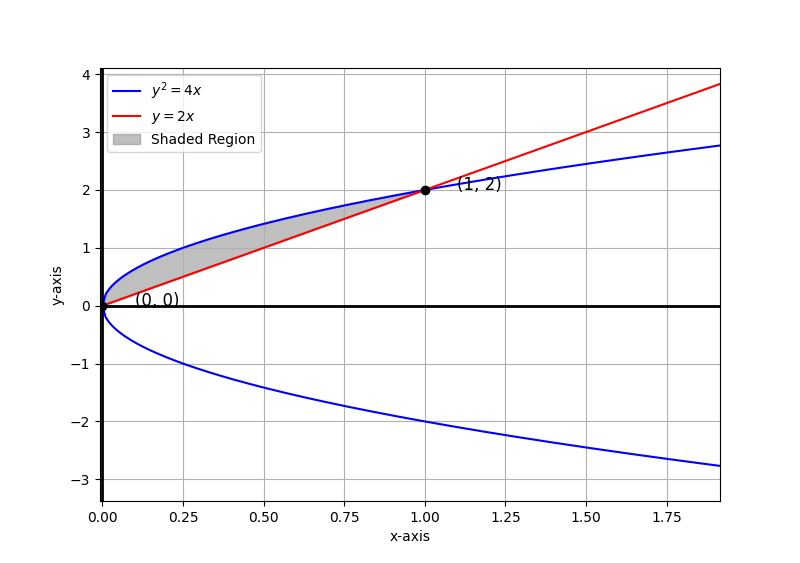
\includegraphics[width=\columnwidth]{fig/Figure_1.png}  
    \caption{Graph}
    \label{fig:example}  % Label for referencing
\end{figure}
  
\end{enumerate}
\end{document}      
